\documentclass[11pt]{article}
\usepackage[margin=1in]{geometry}
\usepackage{amsmath,amssymb,amsfonts}
\usepackage{graphicx}
\usepackage{booktabs}
\usepackage{hyperref}
\usepackage{float}
\usepackage{multirow}
\title{Spectral Clustering: Theory, Algorithm, and Experiments}
\author{Project writeup scaffold}
\date{}

\begin{document}
\maketitle

\section{Introduction}
Spectral clustering is a graph-based clustering method that is especially effective when the geometry of the clusters is non-convex or when Euclidean centroids are a poor summary of the data. The core idea is to convert data points into a weighted graph, study the graph Laplacian, and recover a low-dimensional embedding from a small number of eigenvectors. Clusters are then extracted from that embedding, typically by $k$-means. The project brief asks for a theory summary, a clear algorithmic description with computational considerations, and experiments on multiple synthetic and real datasets, including comparisons with $k$-means and stress tests under noise. This report follows that structure.

\section{Theory summary}
We focus on the normalized spectral clustering algorithm of Ng, Jordan, and Weiss \cite{ng2001spectral}, while relating it to the normalized cut viewpoint of Shi and Malik \cite{shi2000normalized} and the broader graph Laplacian framework summarized by von Luxburg \cite{vonluxburg2007tutorial}.

Given data points $x_1,\dots,x_n$, construct a weighted undirected graph with affinity matrix $W \in \mathbb{R}^{n\times n}$, where $W_{ij}$ is large when $x_i$ and $x_j$ are similar. Let $D$ be the diagonal degree matrix with entries $D_{ii}=\sum_j W_{ij}$. The symmetric normalized Laplacian is
\[
L_{\mathrm{sym}} = I - D^{-1/2} W D^{-1/2}.
\]
The bottom eigenvectors of $L_{\mathrm{sym}}$ reveal approximate connected components or nearly disconnected subgraphs. Intuitively, if the graph consists of $k$ well-separated clusters, then there are $k$ small eigenvalues and the corresponding eigenvectors are approximately piecewise constant on those clusters.

This picture connects to the normalized cut objective. For a partition $A_1,\dots,A_k$, one wants low cross-cluster weight but also avoids trivial solutions by normalizing by cluster volume. The continuous relaxation of this discrete partitioning problem leads to an eigenvector problem involving the normalized Laplacian. This is the main conceptual reason spectral clustering works.

Relative to classical $k$-means, the advantage is that the graph can encode local geometry, so curved manifolds such as the two-moons or concentric-circles datasets are no longer forced into convex Voronoi cells in the original feature space.

\section{Algorithm}
We implement the Ng--Jordan--Weiss algorithm.

\paragraph{Input.} Data matrix $X \in \mathbb{R}^{n\times d}$, number of clusters $k$, number of neighbors $m$ for graph construction.

\paragraph{Output.} Cluster labels $\hat y_1,\dots,\hat y_n$.

\paragraph{Steps.}
\begin{enumerate}
    \item Construct a weighted $m$-nearest-neighbor graph. In our implementation, if $x_j$ is among the $m$ nearest neighbors of $x_i$, the edge weight is
    \[
    W_{ij}=\exp\!\left(-\gamma \|x_i-x_j\|_2^2\right),
    \]
    with $\gamma$ chosen from the median nonzero neighbor distance.
    \item Symmetrize the graph by $W\leftarrow \max(W,W^\top)$.
    \item Form $L_{\mathrm{sym}} = I-D^{-1/2}WD^{-1/2}$.
    \item Compute the eigenvectors corresponding to the $k$ smallest eigenvalues of $L_{\mathrm{sym}}$ and stack them row-wise into $U\in\mathbb{R}^{n\times k}$.
    \item Normalize each row of $U$ to unit norm, obtaining $Y$.
    \item Run $k$-means on the rows of $Y$.
\end{enumerate}

\paragraph{Computational cost.}
If the graph is dense, building all pairwise distances costs $O(n^2 d)$ and storing the affinity matrix costs $O(n^2)$. With a sparse $m$-NN graph, storage drops to $O(mn)$. The dominant linear algebra cost is computing the first $k$ eigenvectors of the normalized Laplacian. For dense methods that is cubic in $n$, but sparse iterative eigensolvers are much cheaper in practice and depend on the number of nonzeros and the spectral gap. The final $k$-means step on the spectral embedding costs roughly $O(nktT)$ where $T$ is the number of Lloyd iterations.

\section{Experimental design}
The brief asks for at least three qualitatively different synthetic examples where the method should work, one or two where it should fail, comparisons to $k$-means, and experiments on real data including noisy variants. We use:
\begin{itemize}
    \item Two moons.
    \item Concentric circles.
    \item Gaussian blobs.
    \item An overlapping-blobs stress case.
    \item Iris data.
    \item A digits subset consisting of classes $\{0,1,3,6\}$.
    \item Zachary's karate club graph.
    \item A noise sweep on the two-moons dataset.
\end{itemize}
We report clustering accuracy after optimal label matching, ARI, NMI, and purity.

\section{Qualitative results}
Figures~\ref{fig:moons}--\ref{fig:digits} show representative synthetic and real-data outcomes. As expected, spectral clustering clearly outperforms $k$-means on non-convex structures such as two moons and circles, while both methods perform competitively on nearly spherical Gaussian blobs. In the overlapping-blobs example, neither method is perfect, illustrating that spectral clustering is not magic: graph construction and the underlying cluster geometry still matter.

\begin{figure}[H]
    \centering
    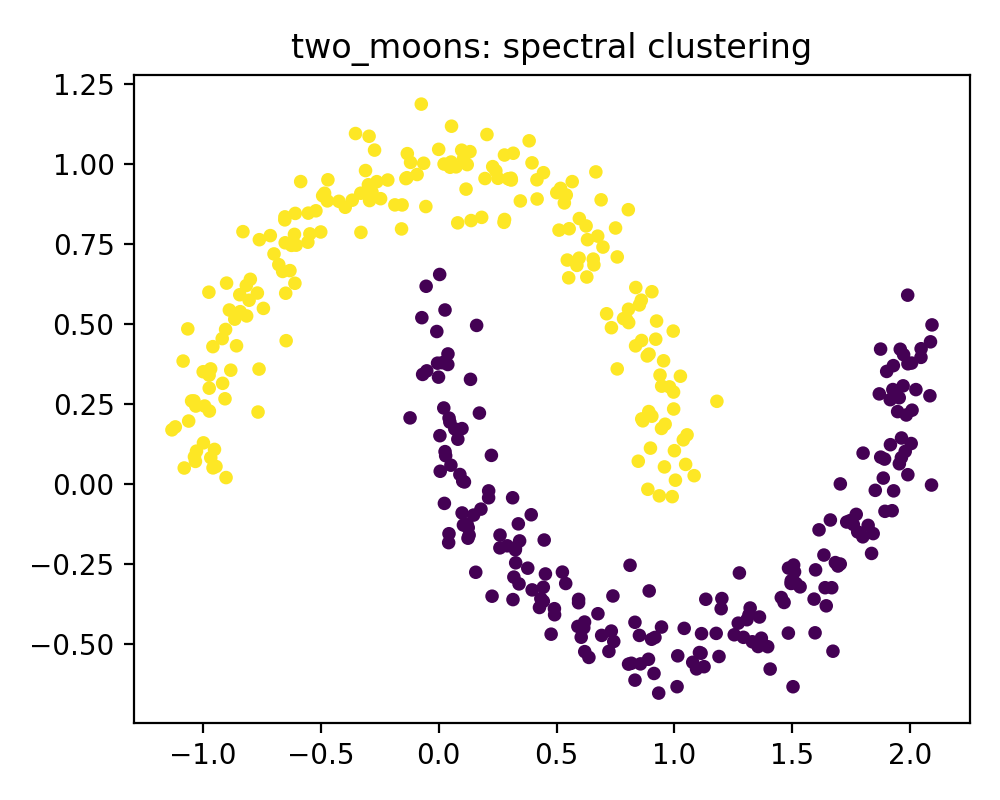
\includegraphics[width=0.47\textwidth]{final_pic/two_moons_spectral.png}
    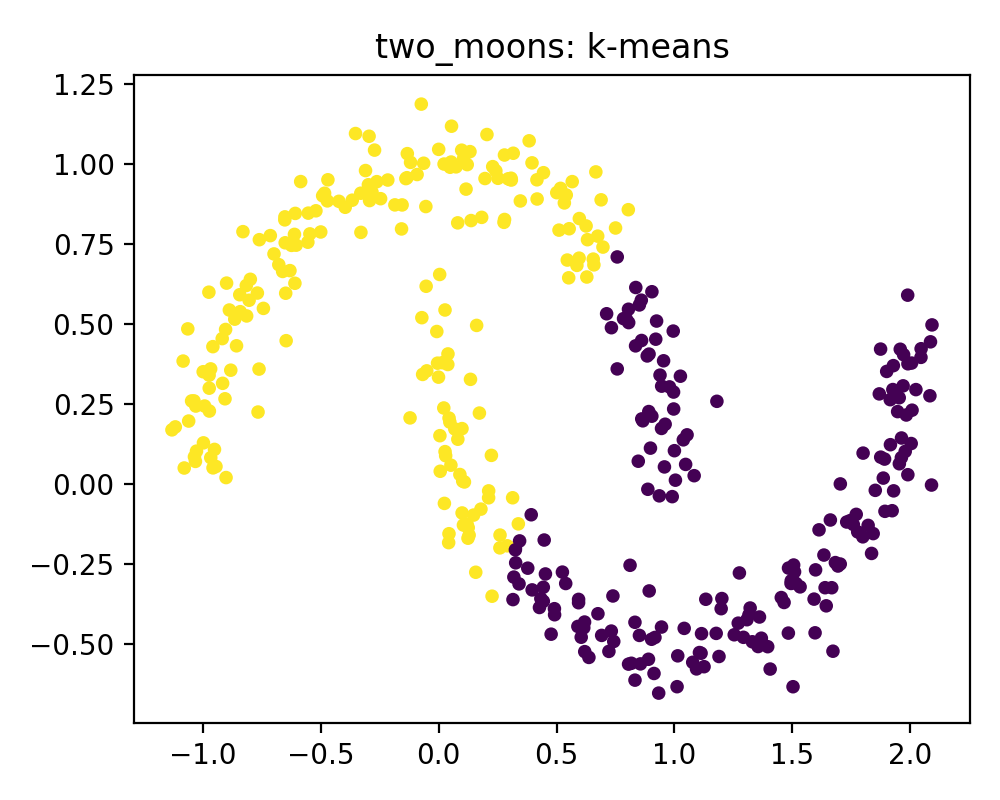
\includegraphics[width=0.47\textwidth]{final_pic/two_moons_kmeans.png}
    \caption{Two moons. Left: spectral clustering. Right: $k$-means. Spectral clustering respects the non-convex geometry much better.}
    \label{fig:moons}
\end{figure}

\begin{figure}[H]
    \centering
    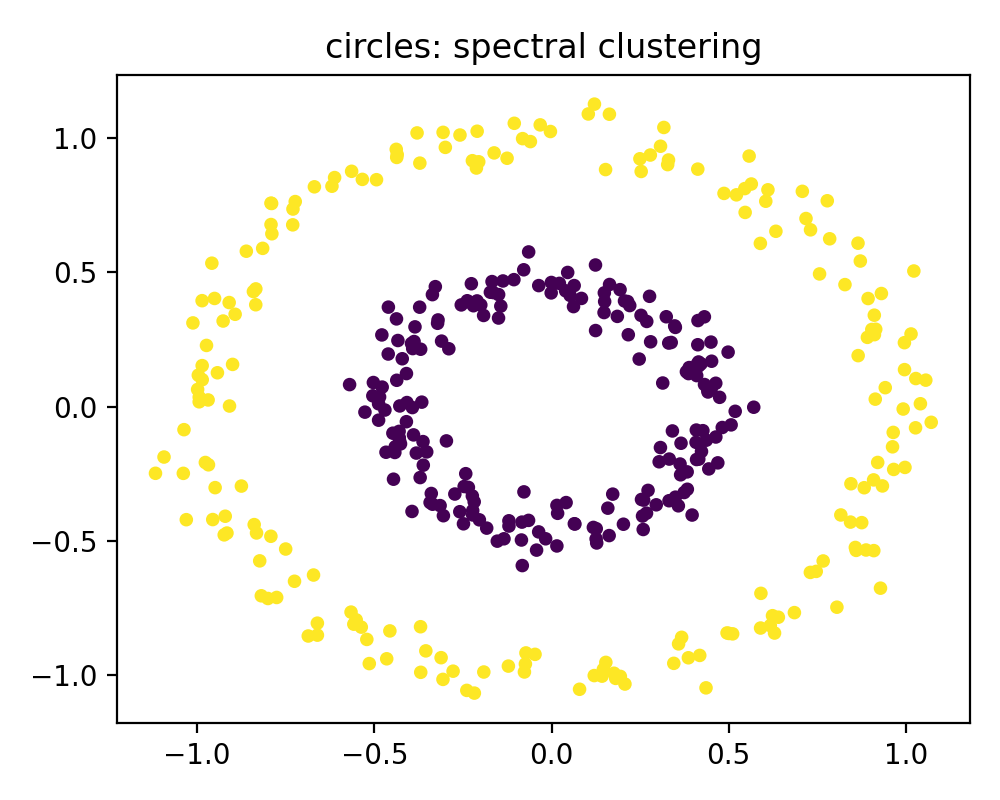
\includegraphics[width=0.47\textwidth]{final_pic/circles_spectral.png}
    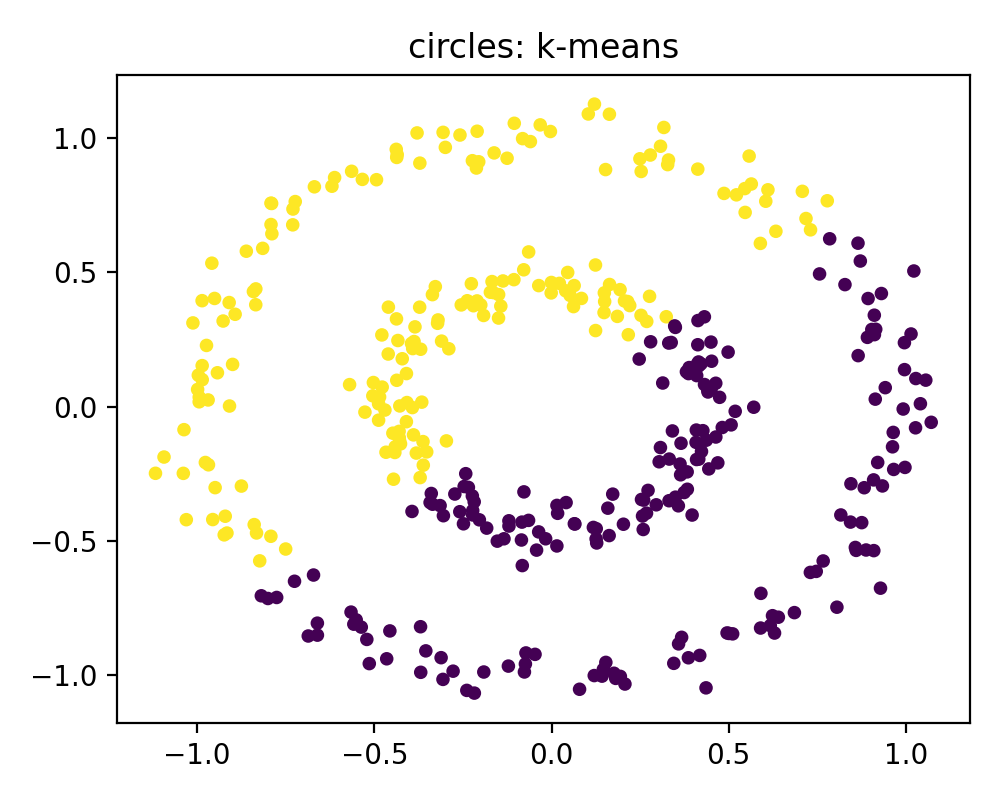
\includegraphics[width=0.47\textwidth]{final_pic/circles_kmeans.png}
    \caption{Concentric circles. Spectral clustering separates the rings, while $k$-means prefers a radial split.}
    \label{fig:circles}
\end{figure}

\begin{figure}[H]
    \centering
    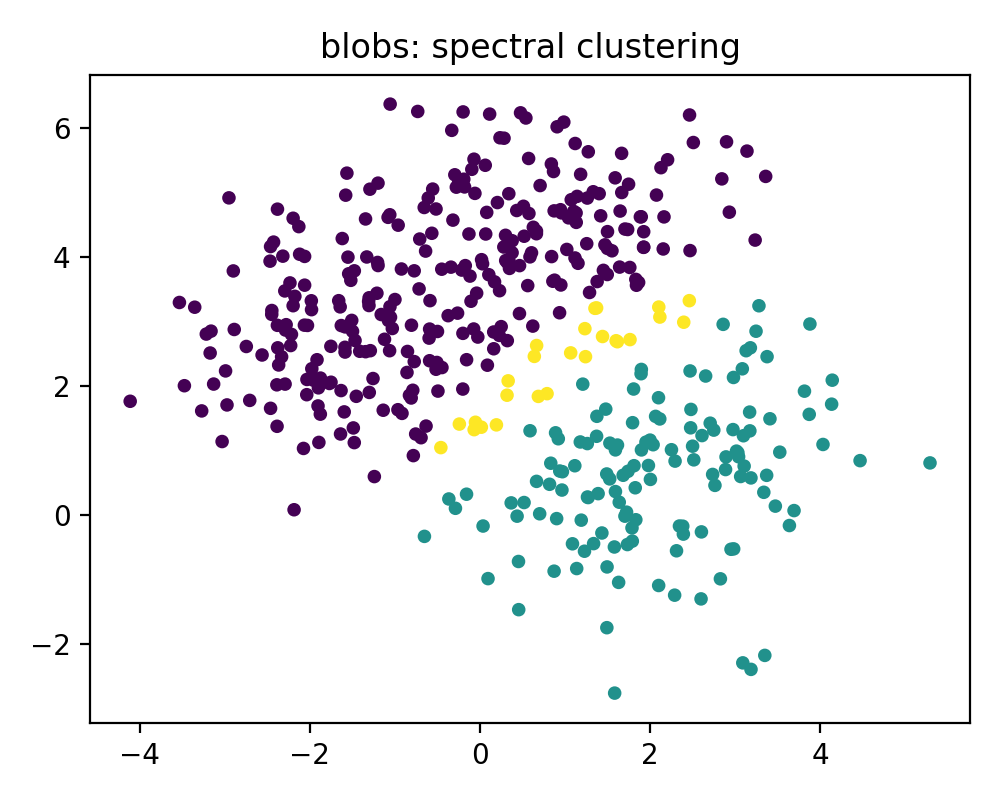
\includegraphics[width=0.47\textwidth]{final_pic/blobs_spectral.png}
    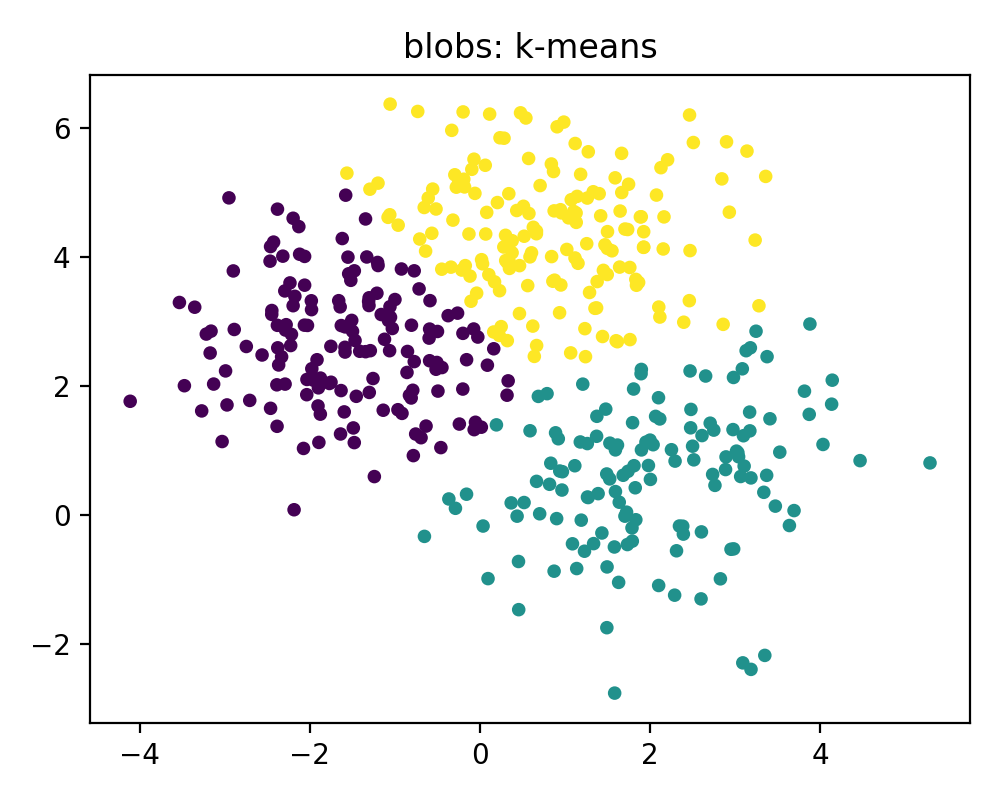
\includegraphics[width=0.47\textwidth]{final_pic/blobs_kmeans.png}
    \caption{Gaussian blobs. Both methods perform well when clusters are close to convex and well-separated.}
    \label{fig:blobs}
\end{figure}

\begin{figure}[H]
    \centering
    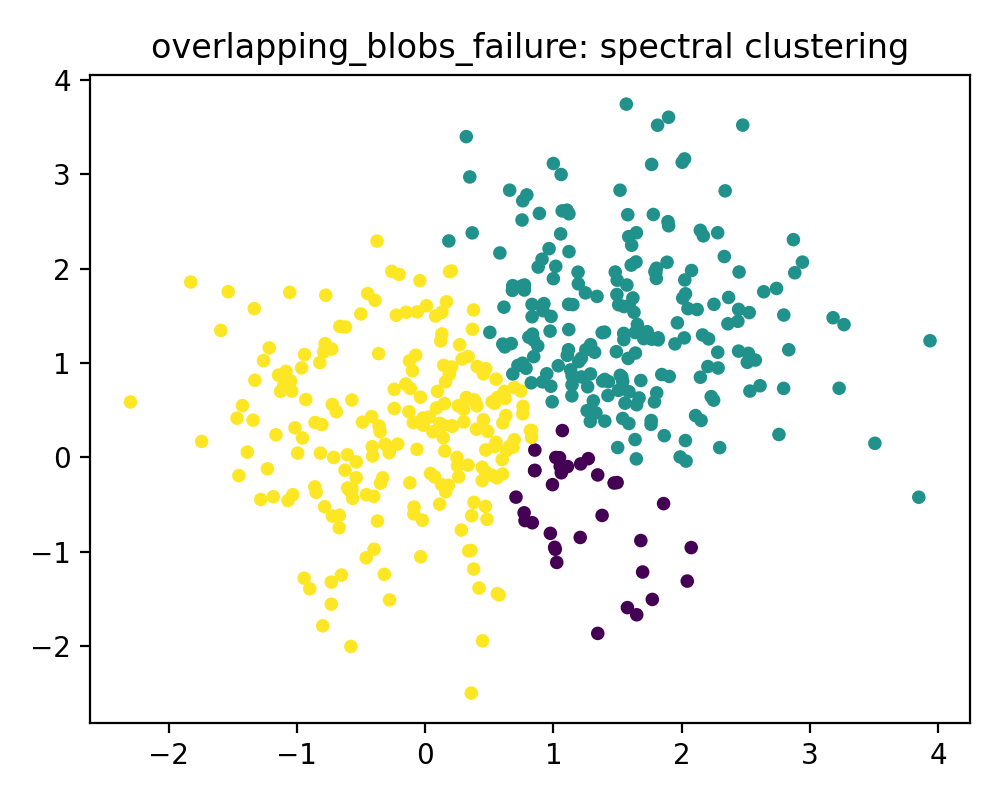
\includegraphics[width=0.47\textwidth]{final_pic/overlapping_blobs_failure_spectral.png}
    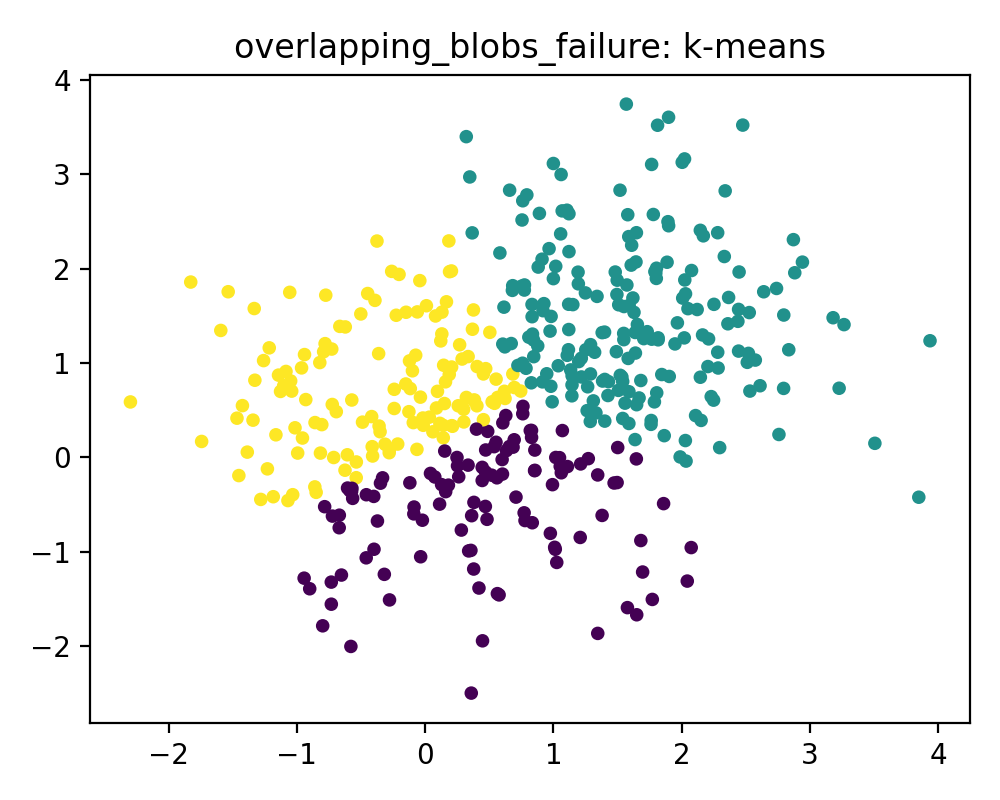
\includegraphics[width=0.47\textwidth]{final_pic/overlapping_blobs_failure_kmeans.png}
    \caption{Overlapping blobs stress case. Performance degrades for both methods, illustrating a regime where no graph construction can fully recover an ambiguous partition.}
    \label{fig:failure}
\end{figure}

\begin{figure}[H]
    \centering
    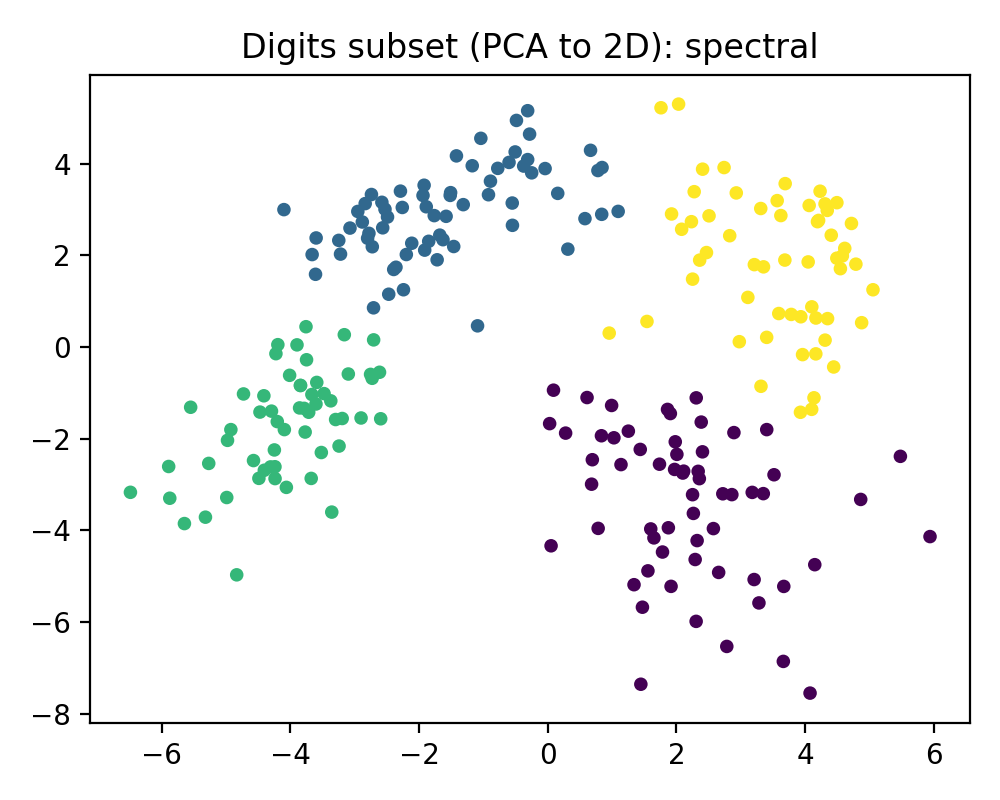
\includegraphics[width=0.47\textwidth]{final_pic/digits_2d_spectral.png}
    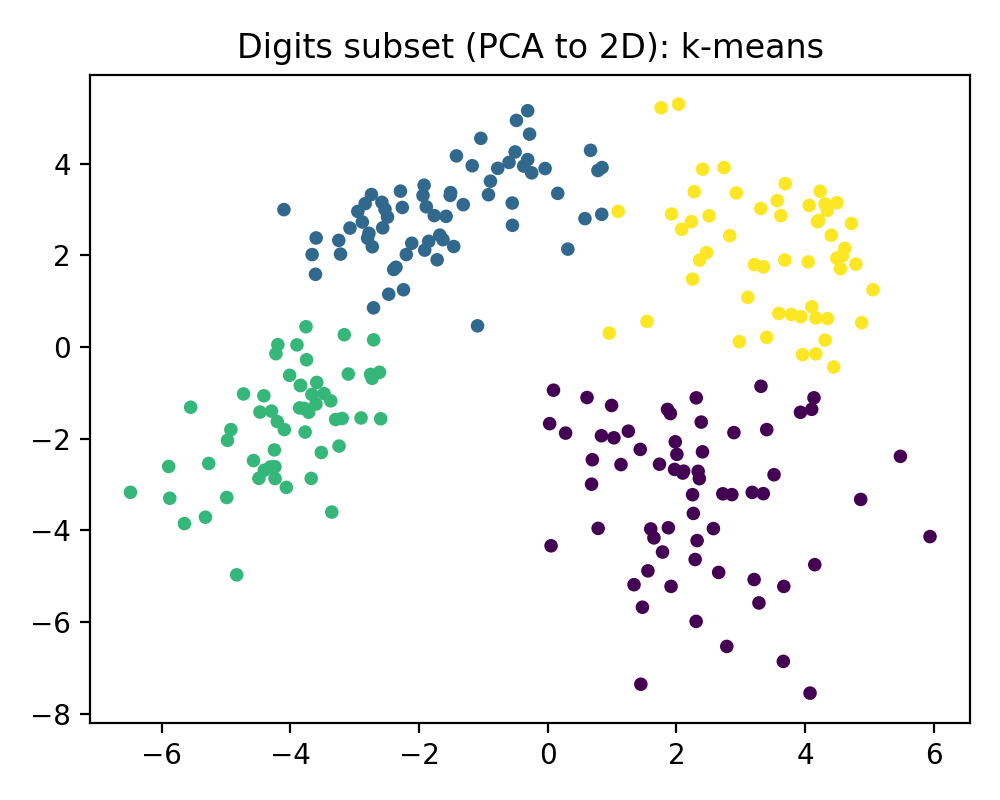
\includegraphics[width=0.47\textwidth]{final_pic/digits_2d_kmeans.png}
    \caption{Digits subset projected to 2D by PCA for visualization only. The actual clustering experiment is run in the original standardized feature space.}
    \label{fig:digits}
\end{figure}

\begin{figure}[H]
    \centering
    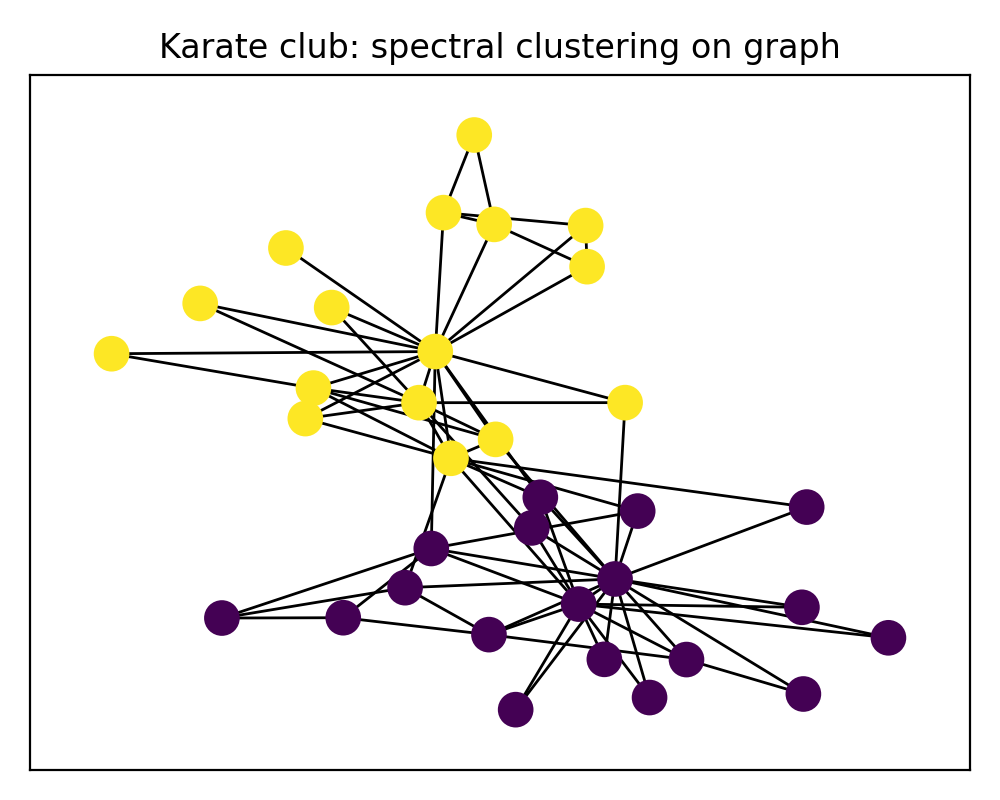
\includegraphics[width=0.6\textwidth]{final_pic/karate_spectral.png}
    \caption{Spectral clustering on Zachary's karate club graph.}
    \label{fig:karate}
\end{figure}

\section{Noise robustness}
Figure~\ref{fig:noise} shows the ARI on the two-moons dataset as isotropic Gaussian noise is increased. Spectral clustering remains clearly better than $k$-means over a useful range of noise levels, although performance eventually degrades as the local neighborhood graph becomes less faithful to the underlying manifold structure.

\begin{figure}[H]
    \centering
    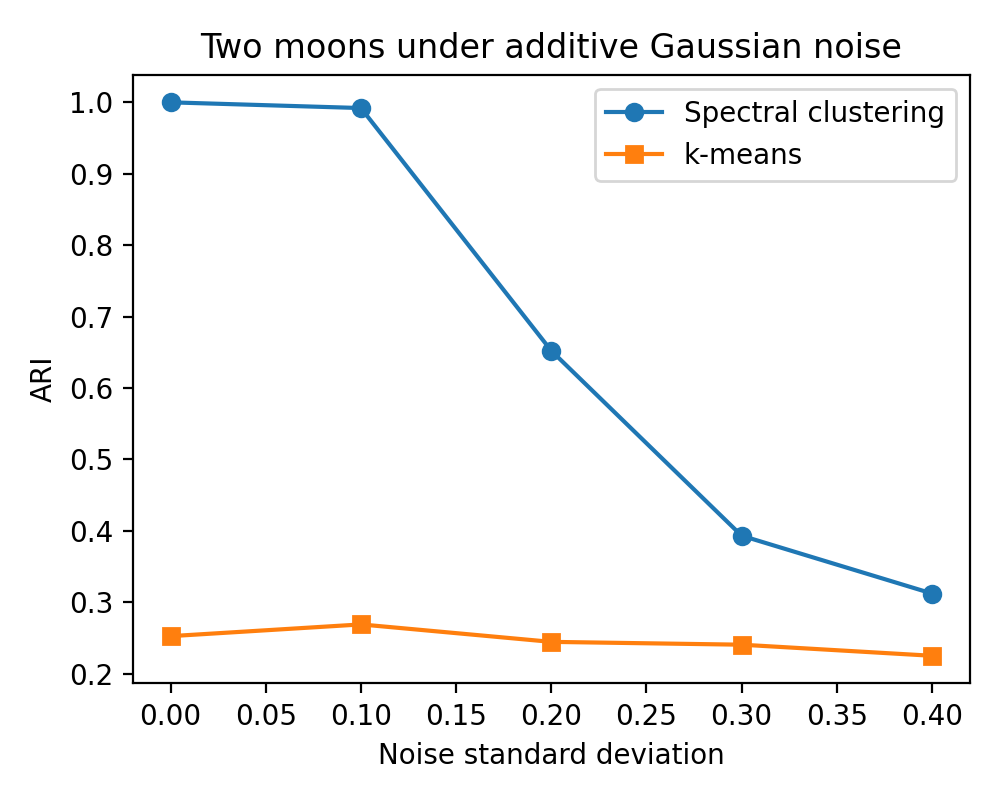
\includegraphics[width=0.6\textwidth]{final_pic/noise_moons_ari.png}
    \caption{ARI versus additive Gaussian noise on the two-moons dataset.}
    \label{fig:noise}
\end{figure}

\section{Discussion}
The experiments align with standard intuition. Spectral clustering is strongest when the data are best viewed through neighborhood relations rather than global Euclidean centroids. It is especially natural for graph data and for feature data with curved or disconnected geometry. Its weaknesses are also visible: graph construction is a modeling choice, the number of neighbors matters, and the eigensolve can become the computational bottleneck on large problems.

The project brief also asks whether the empirical outcomes match expectations. The answer is mostly yes. Two moons and circles are canonical success cases, Gaussian blobs are a regime where $k$-means is already strong, and overlapping blobs give a partial failure case. On the real datasets, the method remains competitive and often stronger than $k$-means, but gains are more modest because class structure is not purely graph-separable.

\section{How to reproduce}
All code is in the `code/` directory. Running `python run_all.py` from that directory regenerates all figures into `final_pic/` and all tables into `results/`. The code is organized into reusable modules for data loading, graph construction, spectral clustering, metrics, plotting, and experiment orchestration.

\bibliographystyle{plain}
\bibliography{refs}

\end{document}
